\documentclass[12pt,letterpaper]{article}
\usepackage{fullpage}
\usepackage[top=2cm, bottom=4.5cm, left=2.5cm, right=2.5cm]{geometry}
\usepackage{amsmath,amsthm,amsfonts,amssymb,amscd}
\usepackage{lastpage}
\usepackage{enumerate}
\usepackage{fancyhdr}
\usepackage{mathrsfs}
\usepackage{xcolor}
\usepackage{graphicx}
\usepackage{listings}
\usepackage{hyperref}
\usepackage{multicol}

\usepackage{enumitem}


\hypersetup{%
  colorlinks=true,
  linkcolor=blue,
  urlcolor=cyan,
  linkbordercolor={0 0 1}
}
 
\renewcommand\lstlistingname{Algorithm}
\renewcommand\lstlistlistingname{Algorithms}
\def\lstlistingautorefname{Alg.}

\lstdefinestyle{Python}{
    language        = Python,
    frame           = lines, 
    basicstyle      = \footnotesize,
    keywordstyle    = \color{blue},
    stringstyle     = \color{green},
    commentstyle    = \color{red}\ttfamily
}

\setlength{\parindent}{0.0in}
\setlength{\parskip}{0.05in}

% Edit these as appropriate
\newcommand\course{PHYS 243}
\newcommand\hwnumber{3}                  % <-- homework number
\newcommand\MyName{TA: Abtin Shahidi}           % <-- My name

\pagestyle{fancyplain}
\headheight 35pt
\lhead{\MyName}

\chead{\textbf{\Large Homework \hwnumber}}
\rhead{\course \\ Deadline:  21 July, 2019, 11:59 pm}
\lfoot{}
\cfoot{}
\rfoot{\small\thepage}
\headsep 1.5em

\begin{document}
\section*{Find the $\pi$ again!}
In the \href{https://abtinshahidi.github.io/teaching/2019-spring-foundation-machine-learning/week3}{week3} course, we discussed how can we find the $\pi$ by just sampling random data points on a square and how to just find the ratio of points inside a circle to total number of generate points. In this week you are going to find the $\pi$ through solving the Buffon's needle problem:

\subsection*{Buffon's needle}
This problem was proposed by a French mathematician named \href{https://en.wikipedia.org/wiki/Georges-Louis_Leclerc,_Comte_de_Buffon}{Georges-Louis Leclerc, Comte de Buffon} in the $18^{th}$ century. Imagine that you have an striped plane as you can see in the picture below and you are throwing a needle on this plane completely randomly. What is the probability of the needle to land fully on a single shade/color. There are two main ways to approach this problem:

\begin{figure}[ht]
\begin{center}
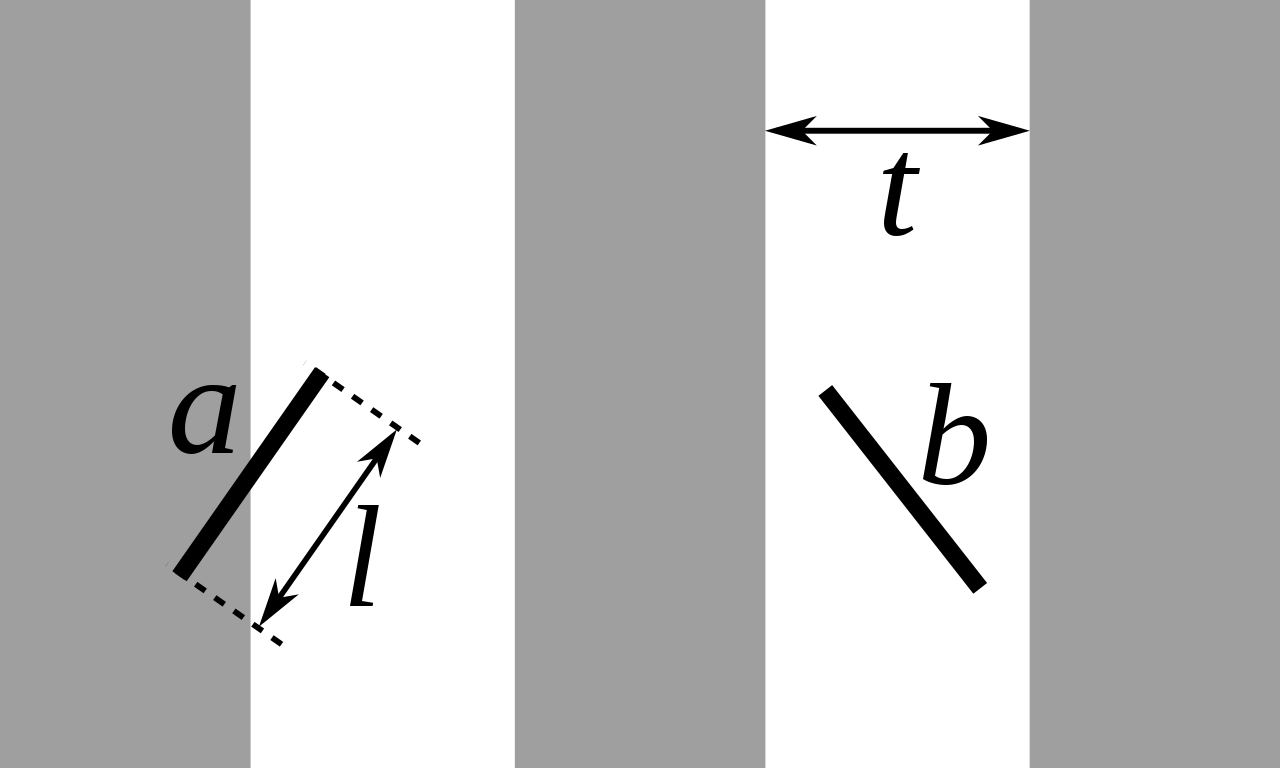
\includegraphics[scale=0.1]{buffon.png}
\end{center}
\caption{Buffon's needle picture from Wikipedia}
\end{figure}

\subsubsection*{Analytic approach:}
For finding the probability let's name stuff, assign probability distribution and possibly taking some integral!

Let the needle length be $l$ and the strip width be $t$. There are two random variables that will determine this probability let's say our random variables are $\theta$ which is the angle of the needle from the direction of strips and $x$ which is the $x$-position of the needles center from the nearest line (this is the one we care each time we drop the needle). Now that we defined our random variables let's assign probability density to them, and since they are two \textbf{independent} variables and they are totally \textbf{random}, we have: 


\begin{multicols}{2}
\noindent
\begin{equation*}
 p(x) = \begin{cases}
 \frac{2}{t} &:\ 0 \le x \le \frac{t}{2}\\
 0 &: \text{elsewhere}
 \end{cases}
\end{equation*}
\begin{equation*}
p(\theta)=
\begin{cases}
\frac{2}{\pi} &:\ 0 \le x \le \frac{\pi}{2}\\
0 &: \text{elsewhere}
\end{cases}
\end{equation*}
\end{multicols}

Since, they are two independent variables I can multiply their probabilities to get their joint probability density distribution: 

\begin{equation*}
p(x,\theta)=
\begin{cases}
\frac{4}{t\pi} &:\ 0 \le x \le \frac{t}{2} , \ 0 \le x \le \frac{t}{2}\\
 0 &: \text{elsewhere}
\end{cases}
\end{equation*}

Now we need to impose are criterion which is coming from the geometry of the problem and can be derived simply to be the following:
\begin{equation*}
l \sin(\theta) \leq t
\end{equation*}

Now we have everything to find the probability, we just need to find the integral which in the case of $l<t$ is:
\begin{equation*}
 P=\int _{\theta =0}^{\frac {\pi }{2}}\int _{x=0}^{(l/2)\sin \theta }{\frac {4}{t\pi }}\,dx\,d\theta ={\frac {2l}{t\pi }}
\end{equation*}

There it is! We have our new formula for $\pi$:

\begin{equation*}
\pi = \frac{2l}{Pt}
\end{equation*}

\begin{enumerate}
\item Find the probability for the case of $l>t$.
\end{enumerate}

\subsubsection*{Numerical simulation:} 
In this part you need to perform a Monte Carlo simulation: \\
\textit{($20\%$ Bonus for Object Oriented implementation)}

\begin{enumerate}[resume]
\item {Find the probability using Monte Carlo simulation for $l<t$, for the general case and find the value of the $\pi$ using some special case (e.g. $l = 2$, and $t = 3$)}  

\item Find the probability using Monte Carlo simulation ($l>t$) for the general case. 


From the probability formula we found for $l<t$, the probability is linear with $l/t$.

\item After writing your general code in \textit{Part 3} plot the Probability vs $l/t$ ratio. \\ 
\textit{\textbf{Hint:} You need to run the simulations for different values of ($l/t$)}


\item Plot the analytic formula for $P(l/t)$ along side your previous result and comment on the result. 
\end{enumerate}

\textit{Clarification : The general case  in this problem means your code should take $l$ and $t$ and produce a probability.}
\end{document}


